\documentclass[pageno]{jpaper}
%replace XXX with the submission number you are given from the ASPLOS submission site.
\newcommand{\asplossubmissionnumber}{XXX}

\usepackage[normalem]{ulem}
\begin{document}

\title{6.867 Machine Learning Homework 2 \& 3}
\date{}
\maketitle

\thispagestyle{empty}


\section{Support Vector Machine Classification}
In this section of the homework we explore the use of support vector machines(SVM) for use in the task of classification. We will focus on implementing the SVM dual optimization problem. Additionally, we will implement the soft-margin SVM which contains a slack variable to allow for data points to be on the incorrect side of the decision boundary with some amount of tolerance. This soft margin allows us to classify points even in the situation when there is no linear separation between classes. This slack is parameterized by the variable C. As C increases the SVM approaches a hard-margin.The complete optimization problem that we seek to solve is shown below.
\begin{figure}[ht!]
\centering
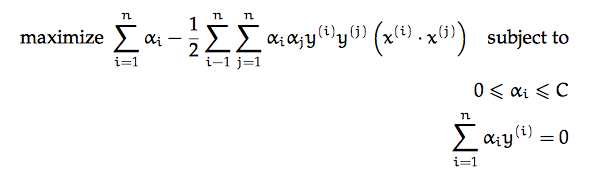
\includegraphics[width=70mm]{svm_dual_soft}
\end{figure}

We utilize the cvxopt quadratic programming toolbox for python in order to solve this convex optimization problem.
Once we optimize for the values of $\alpha$\ we must solve for $w_0$\ and $w$\, shown in the equations below. In the equation below M is the set of support vectors.

\begin{figure}[ht!]
\centering
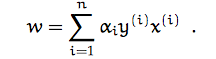
\includegraphics[width=30mm]{w}
\end{figure}

\begin{figure}[ht!]
\centering
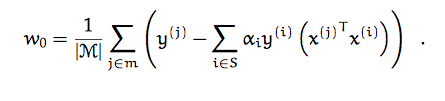
\includegraphics[width=60mm]{W_0}
\end{figure}

After computing $w_0$\ and $w$\ we have our decision boundary and apply the decision rule below to predict the label for subsequent data.

\begin{figure}[ht!]
\centering
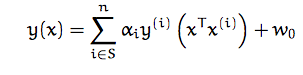
\includegraphics[width=40mm]{decision_rule}
\end{figure}

\subsection{}
In this section we test our implementation of the soft-margin SVM using the synthetic data with positive examples (1, 2), (2, 2) and negative examples (0, 0), (-2, 3). Table 1 shows the alphas resulting from solving the quadratic optimization problem, the Weight and W\_0 vectors as well as the accuracy of this classifier on the training set which is 100\%. Figure one shows the resulting decision boundary and classification of points. We can clearly see that our implementation is successful in producing the maximum margin separator for the training data.
\begin{table}[h!]
  \centering
  \begin{tabular}{llllll|}
    \hline
    \textbf{Alphas}  & \textbf{W}  & \textbf{W\_0} & \textbf{Accuracy}\\
    \hline
    \hline
 5.30612273e-01 	&0.85714299 &-1.21428584   &100\% \\
 \hline
3.11022745e-08	&0.57142862 	& & \\
 \hline
3.67346975e-01	& 	& & \\
 \hline
1.63265328e-01	& 	& & \\
 \hline
  \end{tabular}
  \caption{Optimal Alpha values, Weight vector, W\_0 vector and accuracy for basic dataset}
  \label{table:formatting}
\end{table}

\begin{figure}[ht!]
\centering
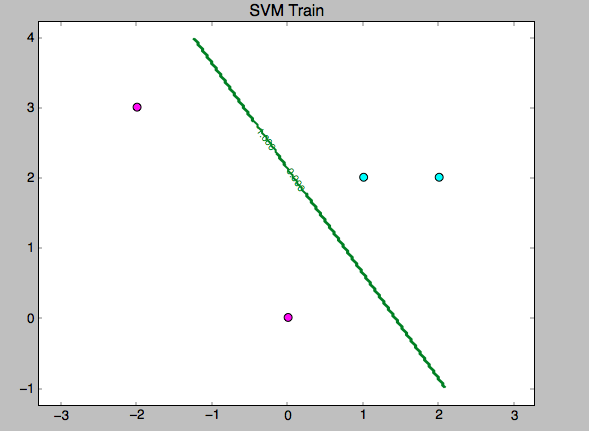
\includegraphics[width=60mm]{1_1_basic_synthetic}
\caption{SVM decision boundary using synthetic data points}
\label{overflow}
\end{figure}

Notice here that none of our $alpha$\ values are zero, yet the data should have produced only three support vectors not four. The model creates a support vector of the point furthest to the right, which is should not; this point should not affect the decision boundary. The value of alpha for this point is very low at 3.11022745e-08. We decided to threshold all alpha values at 1e-5; anything below this value is set to zero.

\subsection{}
C = 1 \\
\begin{figure}[ht!]
\centering
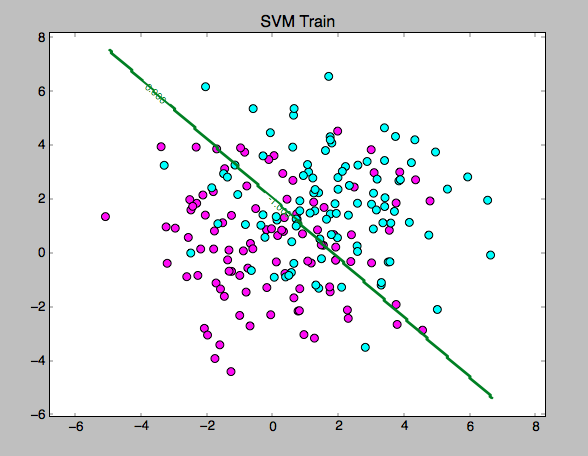
\includegraphics[width=60mm]{bigOverlap_train}
\caption{BigOverlap Data Training}
\label{overflow}
\end{figure}

\begin{figure}[ht!]
\centering
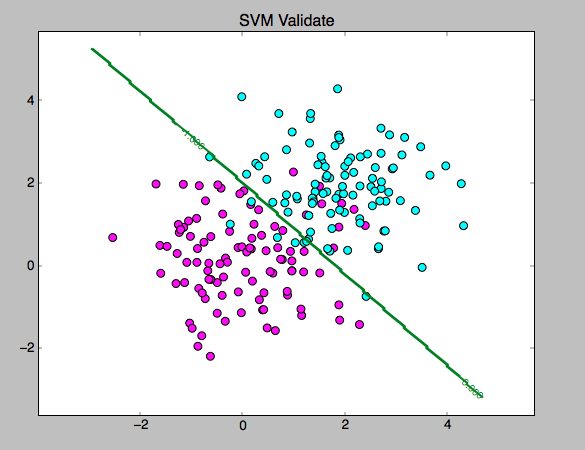
\includegraphics[width=60mm]{bigOverlap_test}
\caption{BigOverlap Data Testing}
\label{overflow}
\end{figure}

\begin{figure}[ht!]
\centering
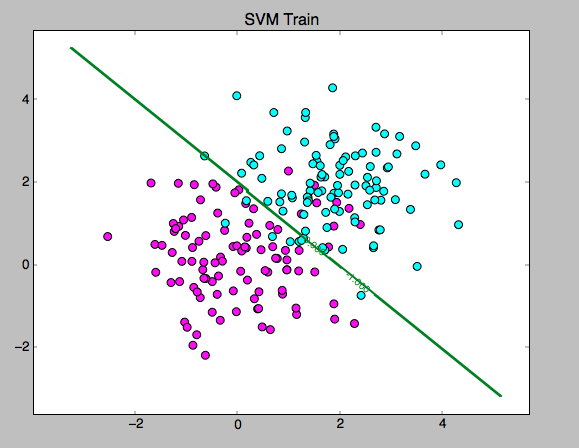
\includegraphics[width=60mm]{smallOverlap_train}
\caption{SmallOverlap Data Training}
\label{overflow}
\end{figure}

\begin{figure}[ht!]
\centering
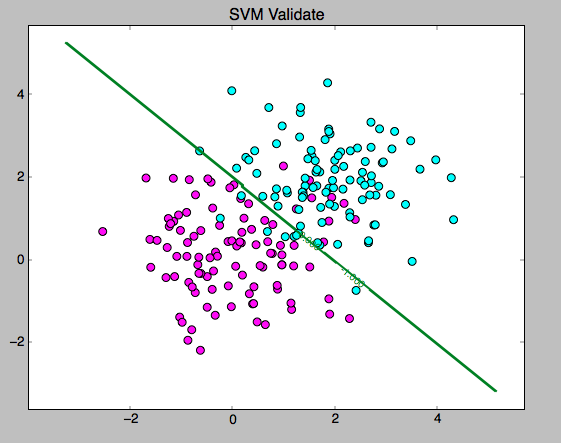
\includegraphics[width=60mm]{smallOverlap_test}
\caption{SmallOverlap Data Testing}
\label{overflow}
\end{figure}

\begin{figure}[ht!]
\centering
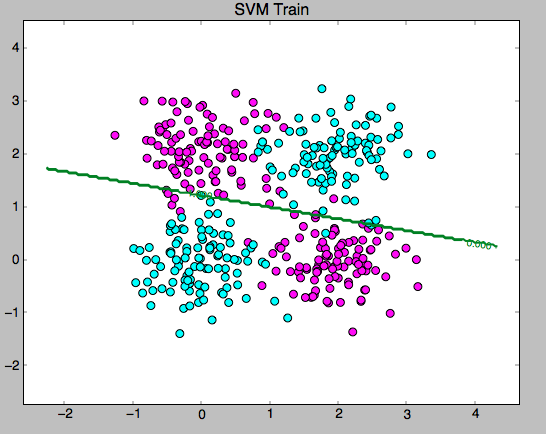
\includegraphics[width=60mm]{nonsep_train}
\caption{Nonsep Data Training}
\label{overflow}
\end{figure}

\begin{figure}[ht!]
\centering
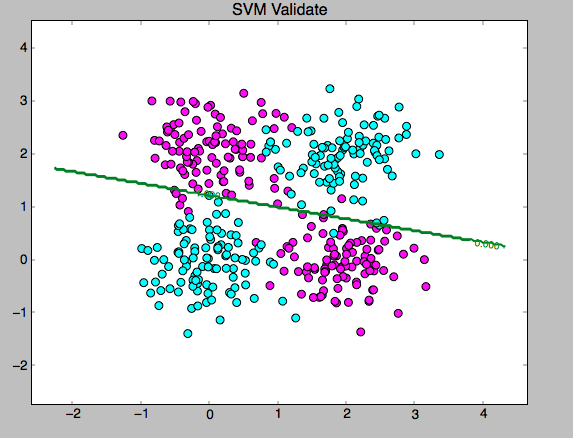
\includegraphics[width=60mm]{nonsep_test}
\caption{Nonsep Data Testing}
\label{overflow}
\end{figure}

\begin{figure}[ht!]
\centering
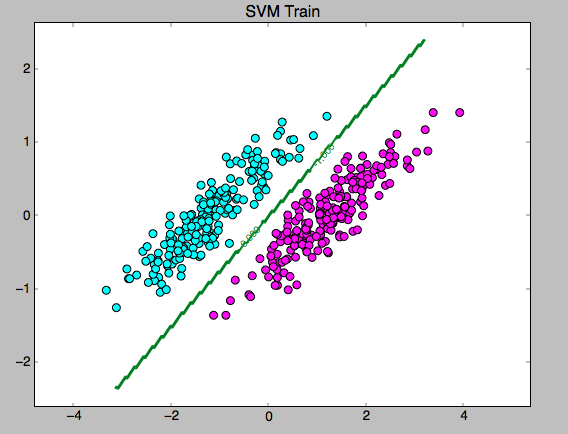
\includegraphics[width=60mm]{ls_train}
\caption{LS Data Training}
\label{overflow}
\end{figure}

\begin{figure}[ht!]
\centering
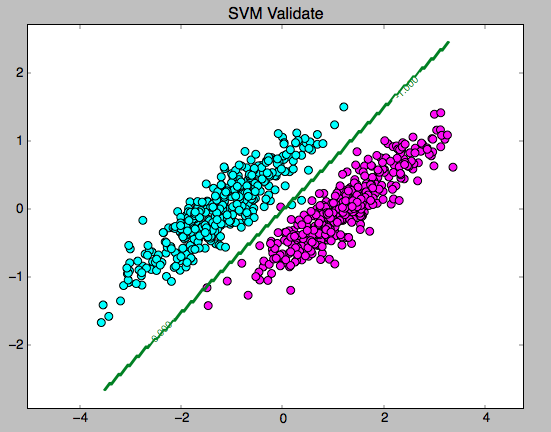
\includegraphics[width=60mm]{ls_test}
\caption{LS Data Testing}
\label{overflow}
\end{figure}



\begin{table}[h!]
  \centering
  \begin{tabular}{llllll|}
    \hline
     \textbf{Data} &\textbf{LS}  & \textbf{Nonsep}  & \textbf{smallOverlap} & \textbf{bigOverlap}\\
    \hline
    \hline
 \textbf{\# Support Vectors} 	&13 &394 &50   &129\%\\
 \hline
\textbf{W}	&-1.94, 2.58 	&  -0.11, -0.51 & 1.12, 1.20 & 0.39, 0.35 \\
 \hline
\textbf{W\_0}	&0.02	&0.61 &-2.36 &-0.70 \\
 \hline
\textbf{Error Train}	&0.00\% 	&0.503\% &0.09\% &0.275\%\\
 \hline
 \textbf{Error Test}	&0.0037\% 	&0.503\% &0.09\% &0.085\%\\
 \hline

  \end{tabular}
  \caption{Number of Support Vectors, Weight vector, W\_0 vector and accuracy for various datasets}
  \label{table:formatting}
\end{table}


\subsection{Problem 1.3}
C vs. geometric margin and alphas 
Beta and some RBF pictures
Try and show the margin on the linear classifier
\section{Logistic Regression}
\section{Multi-Class Classification}



\end{document}

Big overlap\\
Train:\\
w\_0 [-0.7048107]\\
w [ 0.39458465  0.35642887]\\

smallOverlap\\
w\_0 [-2.34573384]\\
w [ 1.21145957  1.2035711 ]\\

ls\\
w\_0 [ 0.01515202]\\
w [-1.94346637  2.57834618]\\

nonsep\\

\begin{table}[h!]

